\documentclass{article}
% Choose a conveniently small page size
% PACKAGES
\usepackage[margin = 1in]{geometry}
\usepackage{amsfonts}
\usepackage{amsmath}
\usepackage{amssymb}
\usepackage{multicol}
\usepackage{graphicx}
\usepackage{float}
\usepackage{xcolor}
\usepackage{amsthm}
\usepackage{dsfont}
\usepackage{hyperref}

% MACROS
% Set Theory
\def\N{\mathbb{N}}
\def\R{\mathbb{R}}
\def\C{\mathbb{C}}
\def\Z{\mathbb{Z}}
\def\^{\hat}
\def\-{\vec}
\def\d{\partial}
\def\!{\boldsymbol}
\def\X{\times}
%\def\-{\bar}
\def\bf{\textbf}
\def\l{\left}
\def\r{\right}
\title{Weekly Report 1}
\author{Damien}
\begin{document}
\maketitle
% \newpage
\section{Progress}
This week I worked on implementing the results in problem 5.1.1 in Kao et al. I made good progress, but the results are still not satisfactory. I describe what I did in detail to help figure out where the problem lies.
\subsection{My Understanding}
I outline here my understanding of sections 2.1.2 and 2.1.3 in Kao et al. that discuss the essential details necessary for implementing problem 5.1.1. The WENO method produces approximations for the fluxes on the cell boundaries. In my implementation I use the third order WENO method. We work on a staggered grid similar to Figure \ref*{fig:grid}.
\begin{figure*}[h]
    \centering
    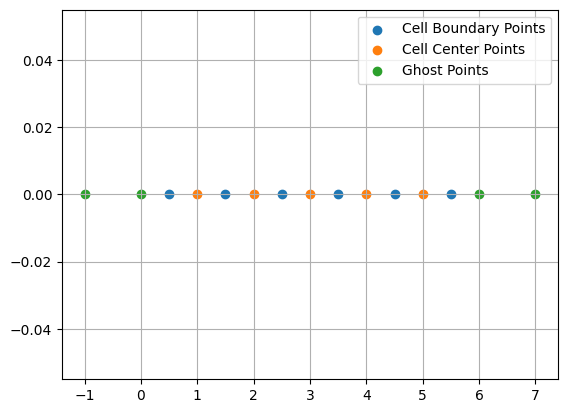
\includegraphics[width=0.5\textwidth]{imgs/grid.png}
    \caption{This figure shows how the grid cells are distributed for the third order WENO scheme. The numbers on the x-axis denote the indices of the points. Since this scheme is third order we have two ghost cells on either side.}
    \label{fig:grid}
\end{figure*}

\noindent The forward fluxes are given by
\begin{equation}\label{eq:f_hat1}
    \^ f_{j + \frac{1}{2}} = w_0 \^ f_{j + \frac{1}{2}}^{(0)} +  w_1 \^ f_{j + \frac{1}{2}}^{(1)} = w_0 \l(\frac{1}{2} f_{j+1} + \frac{1}{2} f_j\r) +  w_1 \l(\frac{3}{2} f_j - \frac{1}{2} f_{j-1}\r).
\end{equation}
Using this, the forward Lax-Friedrichs WENO flux is
\begin{equation*}
    \^{\^{f}}_{j + \frac{1}{2}} = \^f_{j + \frac{1}{2}} + \frac{\sigma}{2}(u_{j+1} - u_j).
\end{equation*}
Putting this all together we get that the forward Lax-Friedrichs WENO sweep is
\begin{align*}
    \frac{(\^{\^{f}}_{j + \frac{1}{2}} - \frac{\sigma}{2}(u_{j+1} - u_j)) - (\^{\^{f}}_{j - \frac{1}{2}} - \frac{\sigma}{2}(u_{j} - u_{j-1}))}{\Delta x} &= s(u_j,x_j) \to \\
    \^{\^{f}}_{j + \frac{1}{2}} - \^{\^{f}}_{j - \frac{1}{2}} - \frac{\sigma}{2}(u_{j+1} - u_j) + \frac{\sigma}{2}(u_{j} - u_{j-1}) &= \Delta x s(u_j,x_j) \to \\
     \sigma (u_{j} - \frac{1}{2}(u_{j+1} + u_{j-1})) &= \Delta x s(u_j,x_j) - (\^{\^{f}}_{j + \frac{1}{2}} - \^{\^{f}}_{j - \frac{1}{2}}) \to \\
     u_{j} &= \frac{1}{2}(u_{j+1} + u_{j-1}) + \frac{1}{\sigma}(\Delta x s(u_j,x_j) - (\^{\^{f}}_{j + \frac{1}{2}} - \^{\^{f}}_{j - \frac{1}{2}})).
\end{align*}
Filling in the values of $\^{\^{f}}_{j + \frac{1}{2}}$ and $\^{\^{f}}_{j - \frac{1}{2}}$ gives
\begin{align*}    
     u_{j} = \frac{1}{2}(u_{j+1} + u_{j-1}) + \frac{1}{\sigma}(\Delta x s(u_j,x_j) - ((\^f_{j + \frac{1}{2}} + \frac{\sigma}{2}(u_{j+1} - u_j)) -  (\^f_{j - \frac{1}{2}} + \frac{\sigma}{2}(u_{j} - u_{j-1})))).
\end{align*}
Filling in the time steps gives
\begin{align*}    
    u^{n+1}_{j} = \frac{1}{2}(u^n_{j+1} + u^{n+1}_{j-1}) + \frac{1}{\sigma}(\Delta x s(u^n_j,x_j) - ((\^f_{j + \frac{1}{2}} + \frac{\sigma}{2}(u^n_{j+1} - u^n_j)) -  (\^f_{j - \frac{1}{2}} + \frac{\sigma}{2}(u^n_{j} - u^{n+1}_{j-1})))).
\end{align*}
Note that if we replaced the $u^{n+1}_{j}$ on the left-hand side with $u^{n+1}_{j}$ we would simply have equality. This method is a non-linear analogue to a simple iteration method. Now, lets look at the backward iteration. The backwards fluxes are given by 
\begin{equation}\label{eq:f_hat2}
    \^ f_{j + \frac{1}{2}} = w_0 \^ f_{j + \frac{1}{2}}^{(0)} +  w_1 \^ f_{j + \frac{1}{2}}^{(1)} = w_0 \l(\frac{1}{2} f_{j} + \frac{1}{2} f_{j + 1}\r) +  w_1 \l(\frac{3}{2} f_{j+1} - \frac{1}{2} f_{j+2}\r).
\end{equation}
Using this, the backwards Lax-Friedrichs WENO flux is
\begin{equation*}
    \^{\^{f}}_{j + \frac{1}{2}} = \^f_{j + \frac{1}{2}} + \frac{\sigma}{2}(u_{j+1} - u_j).
\end{equation*}
We use this to get the backwards Lax-Friedrichs WENO sweep.
\begin{equation*}
    u_{j} = \frac{1}{2}(u_{j+1} + u_{j-1}) + \frac{1}{\sigma}(\Delta x s(u_j,x_j) - (\^{\^{f}}_{j + \frac{1}{2}} - \^{\^{f}}_{j - \frac{1}{2}})).
\end{equation*}
Filling in the values of $\^{\^{f}}_{j + \frac{1}{2}}$ and $\^{\^{f}}_{j - \frac{1}{2}}$ gives
\begin{align*}    
     u_{j} = \frac{1}{2}(u_{j+1} + u_{j-1}) + \frac{1}{\sigma}(\Delta x s(u_j,x_j) - ((\^f_{j + \frac{1}{2}} + \frac{\sigma}{2}(u_{j+1} - u_j)) -  (\^f_{j - \frac{1}{2}} + \frac{\sigma}{2}(u_{j} - u_{j-1})))).
\end{align*}
Filling in the time steps gives
\begin{align*}    
    u^{n+1}_{j} = \frac{1}{2}(u^{n+1}_{j+1} + u^n_{j-1}) + \frac{1}{\sigma}(\Delta x s(u^n_j,x_j) - ((\^f_{j + \frac{1}{2}} + \frac{\sigma}{2}(u^{n+1}_{j+1} - u^n_j)) -  (\^f_{j - \frac{1}{2}} + \frac{\sigma}{2}(u^n_{j} - u^n_{j-1})))).
\end{align*}
Specifically for problem 5.1.1, I set the values on the ghost cells to be zero to enforce the dirichlet boundary conditions.
\subsection*{What I Implemented}
I was a bit confused at first, so the method I originally implemented was the the following. I know this is not the method that they are proposing in the paper, but bear with me briefly. Let $\alpha = \max_u |f'(u)|$. The forward sweep is 
\begin{align*}
    u^{n+1}_{j} = u^n_j - \frac{\Delta t}{\Delta x} (\^f^+_{j + \frac{1}{2}} - \^f^+_{j - \frac{1}{2}}) + \Delta t s(u^n_j,x_j)
\end{align*}
where
\begin{equation*}
    \^f^+_{j + \frac{1}{2}} = \frac{1}{2}(\^f_{j + \frac{1}{2}} + \alpha u)
\end{equation*}
and $\^f_{j + \frac{1}{2}}$ is defined using Equation \ref{eq:f_hat1}. The backwards sweep is 
\begin{align*}
    u^{n+1}_{j} = u^n_j - \frac{\Delta t}{\Delta x} (\^f^-_{j + \frac{1}{2}} - \^f^-_{j - \frac{1}{2}}) + \Delta t s(u^n_j,x_j)
\end{align*}
where
\begin{equation*}
    \^f^-_{j + \frac{1}{2}} = \frac{1}{2}(\^f_{j + \frac{1}{2}} + \alpha u)
\end{equation*}
and $\^f_{j + \frac{1}{2}}$ is defined using Equation \ref{eq:f_hat2}. I applied this method to problem 5.1.1 and got the following plots. 
\begin{figure*}[h]
    \centering
    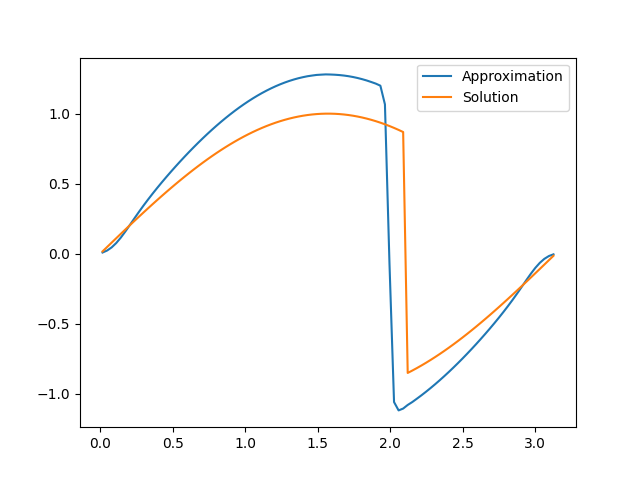
\includegraphics[width=0.5\textwidth]{imgs/sol1.png}
    \caption{Problem 5.1.1 with initial condition $u(x,0) = \beta \sin(x)$ where $\beta = \frac{1}{2}$.}
    \label{fig:sol1}
\end{figure*}
\begin{figure*}[h]
    \centering
    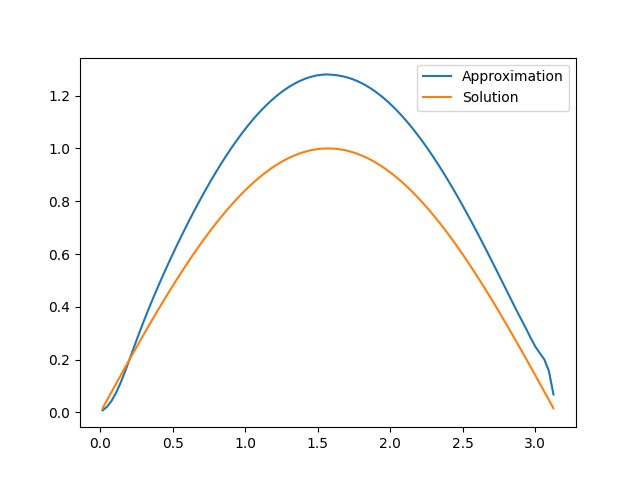
\includegraphics[width=0.5\textwidth]{imgs/sol3.png}
    \caption{Problem 5.1.1 with initial condition $u(x,0) = \beta \sin(x)$ where $\beta = 2$.}
    \label{fig:sol2}
\end{figure*}
This is obviously not the desired method, but it shows that I am on the right track. I am not sure if the difference between the true solution and the approximation is due to numerical issues or whether there is a problem with my implementation. 
\subsection*{Fixing My Mistake}
Once I realized this was not the method I was supposed to implement I tried to adjust the code I had written to match the Lax-Friedrichs WENO sweeping method outlined in section 2.1.3. However, the method does not currently run. There is probably some error baked into the implementation that I am missing so I am going to implement the method from scratch next week. However, I understand the paper much better now so hopefully it will work this time.
\subsection*{Miscellaneous}
I have begun re-reading Finite Volume Methods by Randy LeVeque to solidify my understanding of numerical methods for hyperbolic equations.
\section{To Do}
Re-implement the method from section 2.1.3 to solve 5.1.1.
\end{document}

% \begin{align*}
%     \frac{(\^{\^{f}}_{j + \frac{1}{2}} - \frac{\sigma}{2}(u^n_{j+1} - u^n_j)) - (\^{\^{f}}_{j - \frac{1}{2}} - \frac{\sigma}{2}(u^n_{j} - u^{n+1}_{j-1}))}{\Delta x} = s(u_j^n,x_j) \to \\
%     \^{\^{f}}_{j + \frac{1}{2}} - \^{\^{f}}_{j - \frac{1}{2}} - \frac{\sigma}{2}(u^n_{j+1} - u^n_j) + \frac{\sigma}{2}(u^n_{j} - u^{n+1}_{j-1}) = \Delta x s(u_j^n,x_j) \to \\
%      \sigma (u^n_{j} - \frac{1}{2}(u^n_{j+1} + u^{n+1}_{j-1})) +  = \Delta x s(u_j^n,x_j) - (\^{\^{f}}_{j + \frac{1}{2}} - \^{\^{f}}_{j - \frac{1}{2}})
% \end{align*}